
\documentclass[12pt]{beamer}
\usepackage{amsmath}
\usepackage{mathtools}
\usepackage{multimedia}
\usepackage{hyperref}


\usefonttheme{professionalfonts} % using non standard fonts for beamer
\usefonttheme{serif} % default family is serif
%\documentclass[12pt]{beamerthemeSam.sty}
\usepackage{epsf}
%\usepackage{pstricks}
%\usepackage[orientation=portrait,size=A4]{beamerposter}
\geometry{paperwidth=160mm,paperheight=120mm}
%DT favorite definitions
\def\LL{\left\langle}	% left angle bracket
\def\RR{\right\rangle}	% right angle bracket
\def\LP{\left(}		% left parenthesis
\def\RP{\right)}	% right parenthesis
\def\LB{\left\{}	% left curly bracket
\def\RB{\right\}}	% right curly bracket
\def\PAR#1#2{ {{\partial #1}\over{\partial #2}} }
\def\PARTWO#1#2{ {{\partial^2 #1}\over{\partial #2}^2} }
\def\PARTWOMIX#1#2#3{ {{\partial^2 #1}\over{\partial #2 \partial #3}} }

\def\rightpartial{{\overrightarrow\partial}}
\def\leftpartial{{\overleftarrow\partial}}
\def\diffpartial{\buildrel\leftrightarrow\over\partial}

\def\BCC{\begin{columns}}
\def\ECC{\end{columns}}
\def\HC{\column{0.5\textwidth}}
\def\BC{\begin{center}}
\def\EC{\end{center}}
\def\BN{\begin{enumerate}}
\def\EN{\end{enumerate}}
\def\BI{\begin{itemize}}
\def\EI{\end{itemize}}
\def\BE{\begin{displaymath}}
\def\EE{\end{displaymath}}
\def\BEA{\begin{eqnarray*}}
\def\EEA{\end{eqnarray*}}
\def\BNEA{\begin{eqnarray}}
\def\ENEA{\end{eqnarray}}
\def\EL{\nonumber\\}

\newcommand{\etal}{{\it et al.}}
\newcommand{\gbeta}{6/g^2}
\newcommand{\la}[1]{\label{#1}}
\newcommand{\ie}{{\em i.e.\ }}
\newcommand{\eg}{{\em e.\,g.\ }}
\newcommand{\cf}{cf.\ }
\newcommand{\BS}{\bigskip}
\newcommand{\etc}{etc.\ }
\newcommand{\atantwo}{{\rm atan2}}
\newcommand{\Tr}{{\rm Tr}}
\newcommand{\dt}{\Delta t}
\newcommand{\op}{{\cal O}}
\newcommand{\msbar}{{\overline{\rm MS}}}
\def\chpt{\raise0.4ex\hbox{$\chi$}PT}
\def\schpt{S\raise0.4ex\hbox{$\chi$}PT}
\def\MeV{{\rm Me\!V}}
\def\GeV{{\rm Ge\!V}}

%AB: my color definitions
%\definecolor{mygarnet}{rgb}{0.445,0.184,0.215}
%\definecolor{mygold}{rgb}{0.848,0.848,0.098}
%\definecolor{myg2g}{rgb}{0.647,0.316,0.157}
\definecolor{A}{rgb}{1.0,0.3,0.3}
\definecolor{B}{rgb}{0.0,1.0,0.0}
\definecolor{C}{rgb}{1.0,1.0,0.0}
\definecolor{D}{rgb}{0.5,0.5,1.0}
\definecolor{E}{rgb}{0.7,0.7,0.7}
\definecolor{abtitlecolor}{rgb}{1.0,1.0,1.0}
\definecolor{absecondarycolor}{rgb}{0.0,0.416,0.804}
\definecolor{abprimarycolor}{rgb}{1.0,0.686,0.0}
\definecolor{Red}           {rgb}{1,0.4,0.4}
\definecolor{Yellow}           {rgb}{1,1,0.0}
\definecolor{Grey}          {cmyk}{.7,.7,.7,0}
\definecolor{Blue}          {cmyk}{1,1,0,0}
\definecolor{Green}         {cmyk}{1,0,1,0}
\definecolor{Brown}         {cmyk}{0,0.81,1,0.60}
\definecolor{Silver}        {rgb}{0.95,0.9,1.0}
\definecolor{Sky}           {rgb}{0.07,0.0,0.2}
\definecolor{Darkbrown}     {rgb}{0.4,0.3,0.2}
\definecolor{Black}         {rgb}{0.0,0.0,0.0}
\definecolor{40Gray}        {rgb}{0.4,0.4,0.5}
\usetheme{Madrid}


\setbeamercolor{normal text}{fg=Silver,bg=Sky}

%AB: redefinition of beamer colors
%\setbeamercolor{palette tertiary}{fg=white,bg=mygarnet}
%\setbeamercolor{palette secondary}{fg=white,bg=myg2g}
%\setbeamercolor{palette primary}{fg=black,bg=mygold}
\setbeamercolor{title}{fg=abtitlecolor}
\setbeamercolor{frametitle}{fg=abtitlecolor}
\setbeamercolor{palette tertiary}{fg=white,bg=Darkbrown}
\setbeamercolor{palette secondary}{fg=white,bg=absecondarycolor}
\setbeamercolor{palette primary}{fg=white,bg=40Gray}
\setbeamercolor{structure}{fg=abtitlecolor}

\setbeamerfont{section in toc}{series=\bfseries}

%AB: remove navigation icons
\beamertemplatenavigationsymbolsempty
\title[The Sun]{
  \textbf {The Sun}}

\author [Astronomy 101]{Astronomy 101\\Syracuse University, Fall 2018\\Walter Freeman}

\date{\today}

\begin{document}



\frame{\titlepage}

\frame{
\BC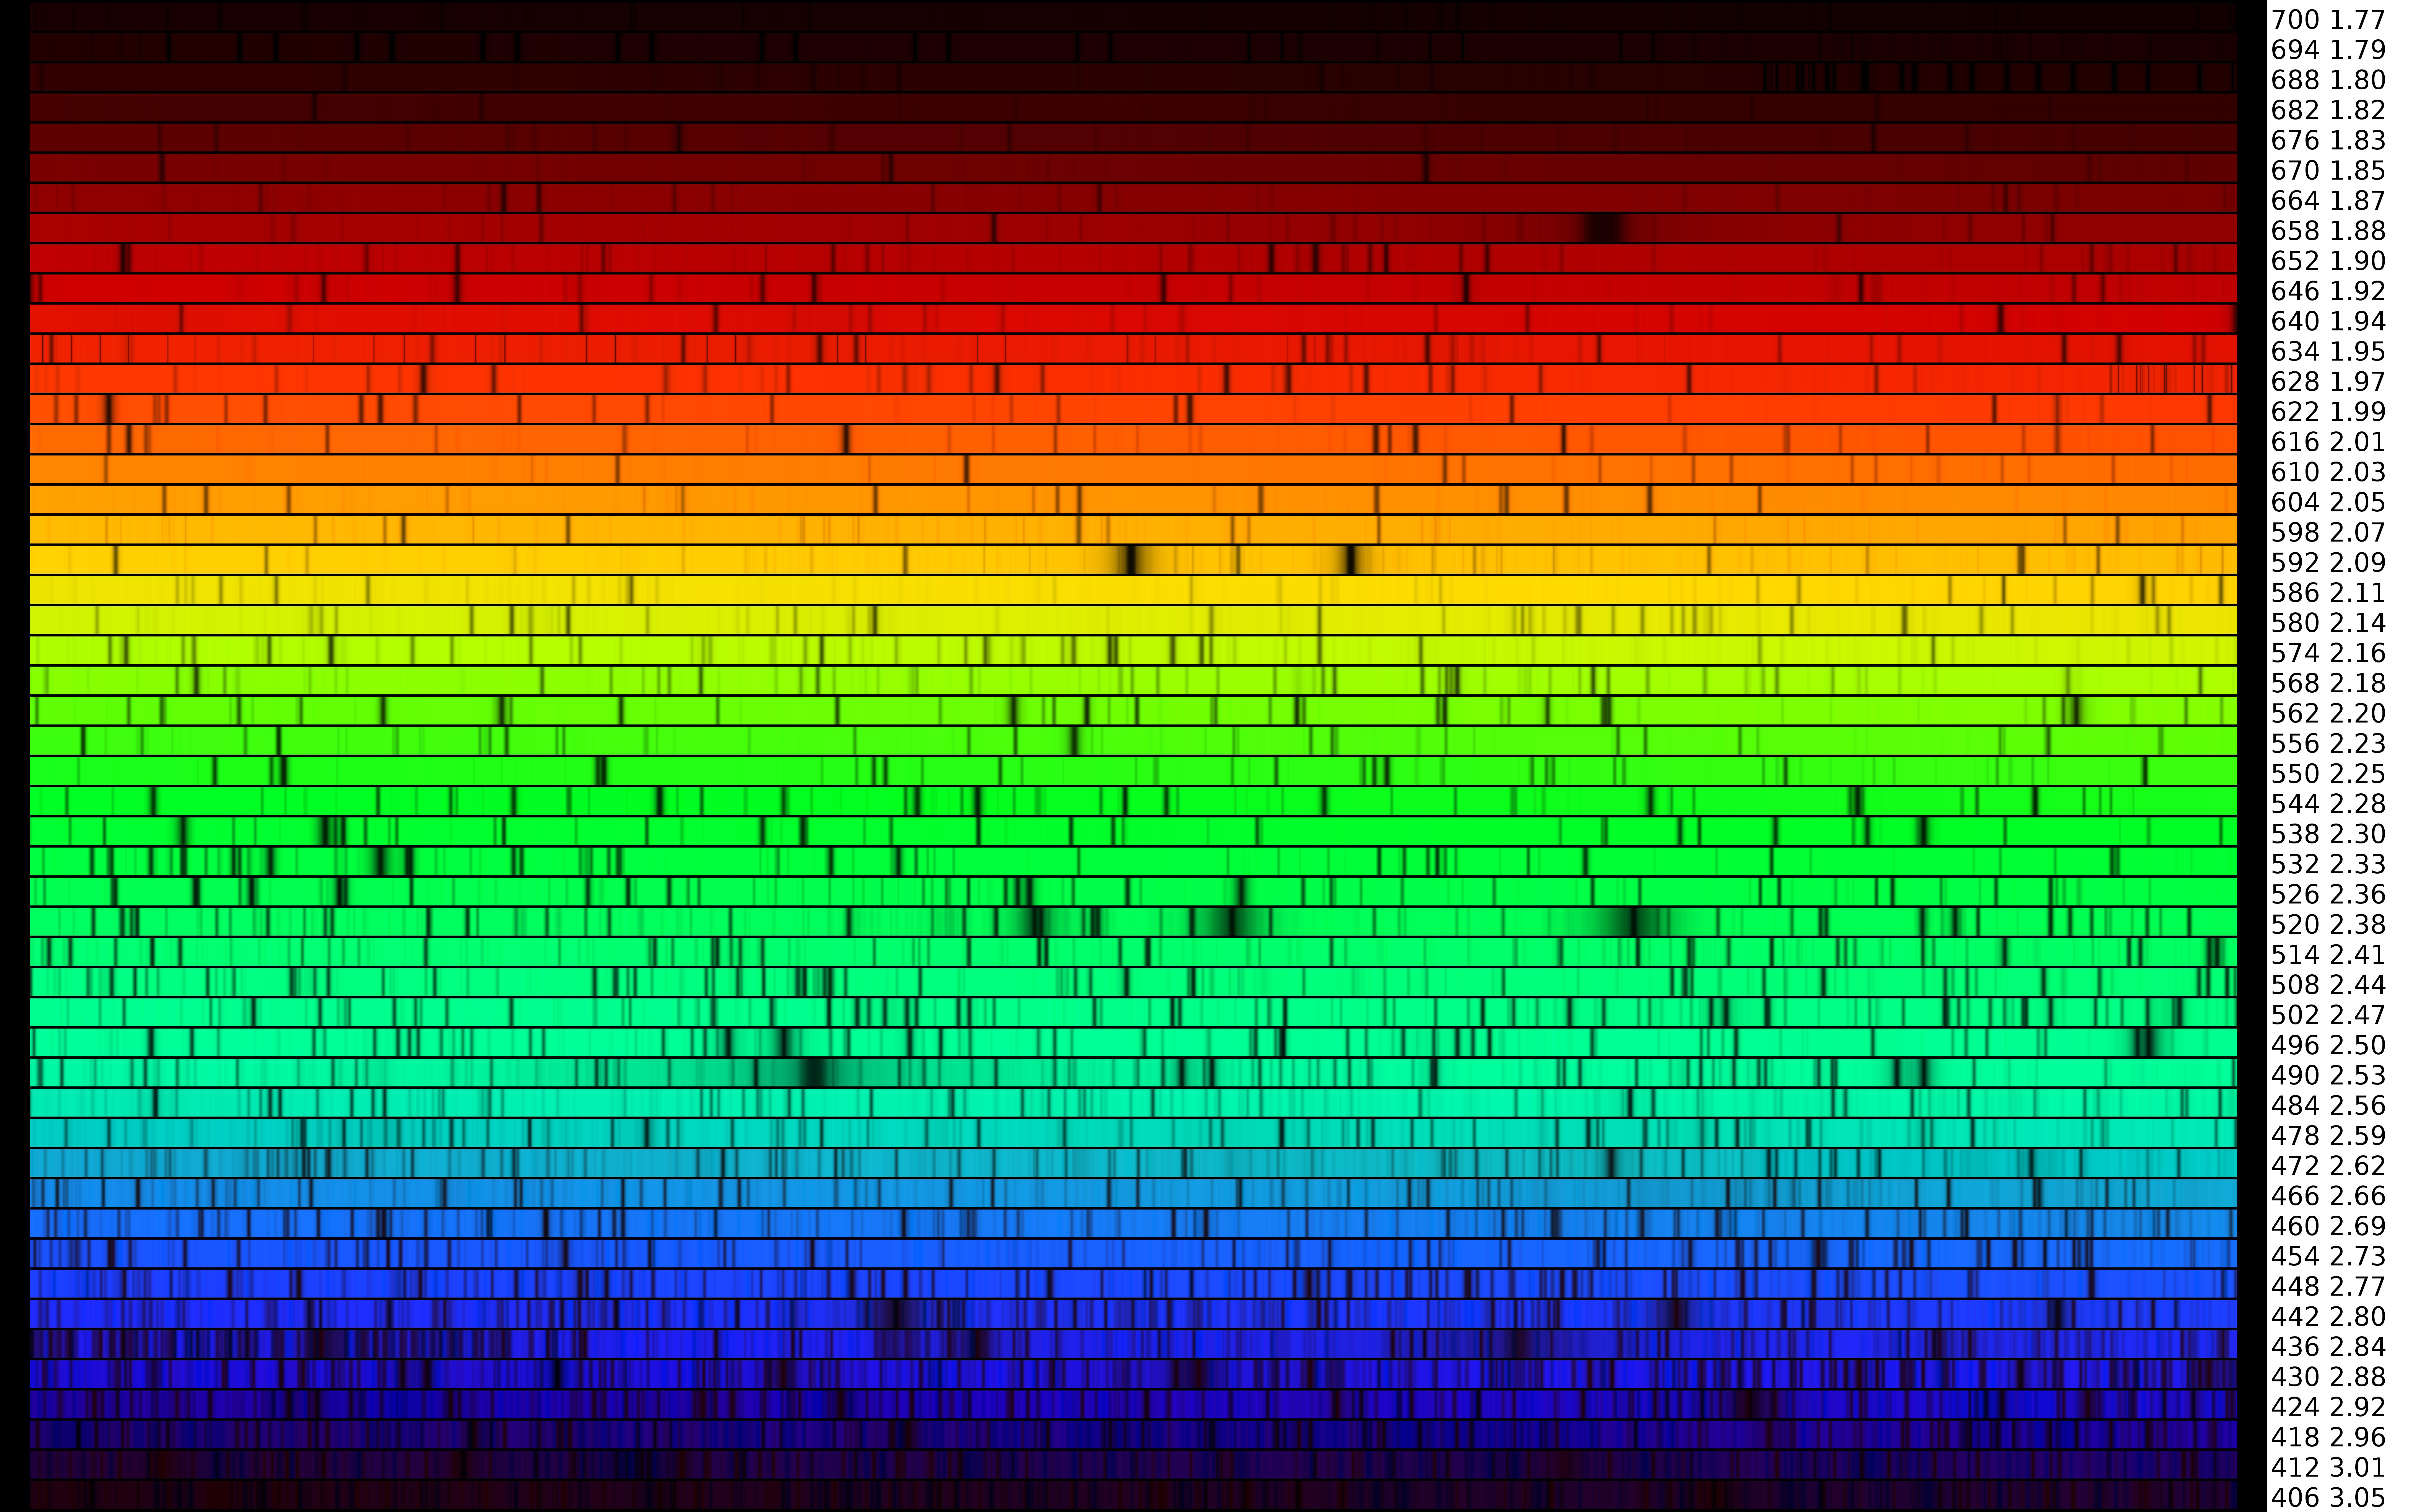
\includegraphics[width=\textwidth]{solarspectrum.jpg}\EC
}

\frame{\frametitle{\textbf{Announcements}}
\Large
\BI
\item Exam 3 on Tuesday
\pause
\item Study guide and last year's exam posted, as usual
\item Solutions to last year's exam will be posted on Friday
\item Extra study sessions (priority for groups): 
\BI
\item Saturday 10AM-1PM, in the Physics Clinic, led by me
\item Sunday 5:45-7:45 PM, in HOL 114, led by Anna
\EI
\pause
\item Grade calculator posted on course website
\EI

}

\frame{
\BC
\includegraphics[height=\textheight]{kepler.jpg}
\EC
}


\frame{\frametitle{\textbf{The Sun's history and the source of its power}}

\BC\includegraphics[width=0.5\textwidth]{hubble-formation.jpg}\\
\small (Hubble Space Telescope image: NASA + ESA / Judy Schmidt)

\BS

Clouds of gas -- mostly hydrogen but with a few heavier elements -- collapse
under their own gravity to form stars.

\EC
}

\frame{\frametitle{\textbf{The Sun's history and the source of its power}}
\Large
\BC
If you smash hydrogen nuclei together hard enough, they fuse to make helium
 -- plus two neutrinos -- plus a {\it lot} of energy.

\BS

$$(P) + (P) + (P) + (P) \rightarrow (NNPP) + 2e^+ + 2\nu$$

How much energy? Let's calculate it!

\pause\BS\BS

This {\color{Red} nuclear fusion} process converts hydrogen fuel into 
helium and a vast amount of energy. Could we harness it here on Earth?
\EC
}

\frame{\frametitle{\textbf{The Sun's fate and the fates of stars}}

\begin{columns}
\column{0.5\textwidth}
\normalsize

\BI
\item When the Sun runs out of hydrogen in its core, the core contracts,
while the outer layers puff up: it becomes a {\color{Red}red giant}. 
(5 billion years in the future, lasting for 1 billion years)

\item Eventually the core gets hot enough to fuse helium
into carbon, and the 
core ignites in a ``helium flash''. 

\item When the helium is depleted, that's it: the Sun isn't heavy enough
to fuse carbon.

\item The carbon core will be left behind as a white dwarf, slowly cooling
-- a dying ember in the sky, called a brown/black dwarf.

\item Its outer layers will be blown out into interstellar space,
briefly forming a nebula.

\EI

\column{0.5\textwidth}

\includegraphics[width=0.9\textwidth]{aldebaran-sun.png}
\footnotesize\it
\BC
(Wikimedia Commons)
\EC

\end{columns}
}


\frame{\frametitle{\textbf{Other stars}}
\BCC
\HC
\includegraphics[width=\textwidth]{hr.png}
\footnotesize\it
\BC
(European Southern Observatory)
\EC
\HC
Most stars are less massive than the Sun.

\BS

These ``red dwarfs'' lead long, cool, boring lives, emitting red and infrared light. 

\BS

They are too faint for
us to see without telescopes, but they contribute to the Milky Way glow.

\BS

They will live 10-100 times as long as the present age of the universe -- a trillion years.

\BS 

They will burn their hydrogen until it is all gone, then slowly fade away as brown dwarfs.

\ECC

}

\frame{\frametitle{\textbf{Other stars}}
\BCC
\HC
\includegraphics[width=\textwidth]{onion-fusion.png}
\BC
\it \footnotesize Wikimedia Commons / R. J. Hall. \\Image not to scale.
\EC
\HC
\small
More massive stars have enough weight to compress their carbon cores and fuse it to neon.

\BS

This process releases less energy than even helium fusion, so it doesn't last as long.

\BS

Elements fuse into heavier and heavier elements, releasing less energy each time, until they reach iron in the 
heaviest stars.

\BS

Iron is ``stellar ash'' -- it can't release any more energy by fusion.

\BS 

In some of these heaviest stars, once their iron cores grow too much, 
gravity crushes them into one enormous atomic nucleus -- a neutron star.


\ECC
}


\frame{\frametitle{\textbf{Supernovae}}
\BCC
\HC
\includegraphics[width=\textwidth]{crab-nebula.jpg}
\BC
\footnotesize\it (Hubble Space Telescope/NASA)
\EC
\HC
\small
The resulting explosion destroys the rest of the star.

\BS
\BS

It causes a flurry of nuclear reactions, forging elements heavier than iron.

\BS

It also scatters the heavy-element-rich contents of the star out to space.
This is why the Earth has so much iron in it -- and where our heavy elements come from.

\BS

It releases massive amounts of energy, forming a bright flash in the sky.

\BS

This is the Crab Nebula, the remnant of the 1054 supernova.

\BS

It was hundreds of times further away than most visible stars, but could be seen even during the day!

\ECC
}





\end{document}

